\section{Analyse von Schaltungen}
Die Übertragungsfunktion von Opamp Schaltungen berechnet sich als 
Summe aller Eingangs-Admittanzen $Y_n$ multipliziert mit der Opamp-Funktion
$\Zop$. 
\begin{multicols}{2}
	\begin{center}
		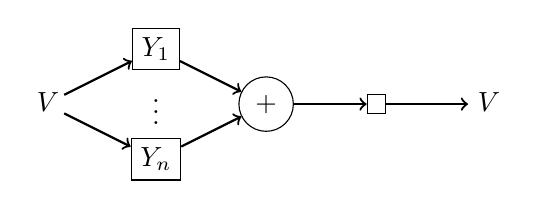
\begin{tikzpicture}[scale=0.7]

% Nodes
\node (vin) at (-2,0) {$V_{\In}$};

\node[rectangle,draw] (y1) at (0,1) {$Y_1$};
\node at (0,0) {$\vdots$};
\node[rectangle,draw] (yn) at (0,-1) {$Y_n$};

\node[circle,draw] (sum) at (2,0) {$+$};
\node[rectangle,draw] (zop) at (4,0) {$\Zop$};
\node (vout) at (6,0) {$V_{\Out}$};

% Connections
\draw[thick,->] (vin) -- (y1);
\draw[thick,->] (vin) -- (yn);

\draw[thick,->] (y1) -- (sum);
\draw[thick,->] (yn) -- (sum);

\draw[thick,->] (sum) -- (zop);
\draw[thick,->] (zop) -- (vout);

\end{tikzpicture}
	\end{center}
	\vfill
	\columnbreak
	\hspace{2cm}
	\begin{equation*}
		T(z) = \sum\limits_{n} Y_{n} \Zop
	\end{equation*}
\end{multicols}

\subsection{Spannung zu Strom}

\begin{tabularx}{\linewidth}{p{0.25\linewidth}XX}
	\textbf{Bezeichnung} & \textbf{Schaltung} & \textbf{Admittanz} \\ \hline
	Widerstand & \begin{circuitikz}[scale=0.7,transform shape]
	\draw
		(0,0) node[anchor=east]{$V_{\In}$} to[R=$R$]  (6,0) node[anchor=west]{$V_{\Out}$}
		;	

\end{circuitikz} & $Y_{r}(s) = \frac{1}{R}$ \\
	Kapazität & \begin{circuitikz}[scale=0.7,transform shape]
	\draw
		(0,0) node[anchor=east]{$V_{\In}$} to[C=$C$]  (6,0) node[anchor=west]{$V_{\Out}$}
		;	

\end{circuitikz} & $Y_{c}(s) = sC$ \\
	Geschaltetes C & \begin{circuitikz}[scale=0.7,transform shape]
	\draw
		(0,0) node[anchor=east]{$V_{\In}$} to[switch={PH0}]  (2,0)
		(2,0) to[switch={PH1},mirror] (2,-1) node[sground,scale=0.7]{}
		(2,0) to[C=$C$] (4,0)
		(4,0) to[switch={PH1}] (4,-1) node[sground,scale=0.7]{}
		(4,0) to[switch={PH0}] (6,0) node[anchor=west]{$V_{\Out}$}
		;	

\end{circuitikz} & $Y_{sc}(s) = \frac{C}{T}$ \\
	Geschaltetes C mit Inversion & \begin{circuitikz}[scale=0.7,transform shape]
	\draw
		(0,0) node[anchor=east]{$V_{\In}$} to[switch={PH0}]  (2,0)
		(2,0) to[switch={PH1}] (2,-1) node[sground,scale=0.7]{}
		(2,0) to[C=$C$] (4,0)
		(4,0) to[switch={PH0}] (4,-1) node[sground,scale=0.7]{}
		(4,0) to[switch={PH1}] (6,0) node[anchor=west]{$V_{\Out}$}
		;	

\end{circuitikz} & $Y_{sc}(s) = -\frac{C}{T}$ \\
	\hline
\end{tabularx}

\subsection{Strom zu Spannung}

\begin{tabularx}{\linewidth}{p{0.25\linewidth}XX}
	\textbf{Bezeichnung} & \textbf{Schaltung} & \textbf{Impedanz} \\ \hline
	Opamp als Verstärker & \begin{circuitikz}[scale=0.7,transform shape]
	\draw

		(0,0) node[op amp] (opamp) {}

		(-2,0.49) node[anchor=east] {$V_{\In}$} to (opamp.-)
		(-1.5,0.49) to[short,*-] (-1.5,1.5)
		(-1.5,1.5) to[R=$R_f$] (1.5,1.5)
		(1.5,1.5) to[short,-*] (1.5,0)
		(opamp.out) to (2,0) node[anchor=west] {$V_{\Out}$}
		(opamp.+) -| (-1.5,-1) node[sground,scale=0.7] {}
				
	;	

\end{circuitikz} & $\Zop = -R_f$ \\
	Opamp als Integrator & \begin{circuitikz}[scale=0.7,transform shape]
	\draw

		(0,0) node[op amp] (opamp) {}

		(-2,0.49) node[anchor=east] {$V_{\In}$} to (opamp.-)
		(-1.5,0.49) to[short,*-] (-1.5,1.5)
		(-1.5,1.5) to[C=$C_f$] (1.5,1.5)
		(1.5,1.5) to[short,-*] (1.5,0)
		(opamp.out) to (2,0) node[anchor=west] {$V_{\Out}$}
		(opamp.+) -| (-1.5,-1) node[sground,scale=0.7] {}
				
	;	

\end{circuitikz} & $\Zop = - \frac{1}{s C_f}$ \\
	Opamp als Tiefpass & \begin{circuitikz}[scale=0.7,transform shape]
	\draw

		(0,0) node[op amp] (opamp) {}

		(-2,0.49) node[anchor=east] {$V_{\In}$} to (opamp.-)
		(-1.5,0.49) to[short,*-] (-1.5,1.5)
		(-1.5,1.5) to[R=$R_f$] (1.5,1.5)
		(-1.5,1.5) to[short,*-] (-1.5,3)
		(1.5,1.5) to[short,*-] (1.5,3)
		(-1.5,3) to[C=$C_f$] (1.5,3)
		(1.5,1.5) to[short,-*] (1.5,0)
		(opamp.out) to (2,0) node[anchor=west] {$V_{\Out}$}
		(opamp.+) -| (-1.5,-1) node[sground,scale=0.7] {}
				
	;	

\end{circuitikz} & $\Zop = - \frac{R_f}{1+s C_f R_f}$  \\
	\hline
\end{tabularx}

\subsection{Rechenregeln Blockdiagramme}

\begin{tabularx}{\linewidth}{p{0.25\linewidth}XX}
	\textbf{Bezeichnung} & \textbf{Schaltung} & \textbf{Berechnung} \\ \hline
	Serieschaltung & \begin{circuitikz}[scale=0.7,transform shape]
	\node[anchor=east] (xs) at (0,0) {$X(s)$};
	\node[draw,rectangle] (t1) at (2,0) {$T_1(s)$};
	\node[draw,rectangle] (t2) at (4,0) {$T_2(s)$};
	\node[anchor=west] (ys) at (6,0) {$Y(s)$};		

	\draw[thick,->] (xs) -- (t1);
	\draw[thick,->] (t1) -- (t2);
	\draw[thick,->] (t2) -- (ys);

	\node at (0,-1) {}; \node at (0,1) {};
\end{circuitikz} & $T(s) = T_1(s) \cdot T_2(s)$ \\
	Parallelschaltung & \begin{circuitikz}[scale=0.7,transform shape]
	\node[anchor=east] (xs) at (0,1) {$X(s)$};
	\node[draw,rectangle] (t1) at (2,1) {$T_1(s)$};
	\node[draw,rectangle] (t2) at (2,-1) {$T_2(s)$};
	\node[anchor=west] (ys) at (6,1) {$Y(s)$};	
	\node[draw,circle,minimum size=0mm,inner sep=2pt] (sum) at (4,1) {$+$};
	\node[circle,fill,inner sep=0pt, minimum size=2mm] (p) at (0.75,1) {};	

	\draw[thick,->] (xs) -- (t1);
	\draw[thick,->] (p) |- (t2.west);
	\draw[thick,->] (t1) -- (sum.west);
	\draw[thick,->] (t2.east) -| (sum.south);
	\draw[thick,->] (sum.east) -- (ys);

\end{circuitikz} & $T(s) = T_1(s) + T_2(s)$ \\
	Rückkopplung & \begin{circuitikz}[scale=0.7,transform shape]
	\node[anchor=east] (xs) at (0,1) {$X(s)$};
	\node[draw,circle,minimum size=0mm,inner sep=2pt] (sum) at (2,1) {$+$};
	\node[draw,rectangle] (t1) at (4,1) {$T_1(s)$};
	\node[draw,rectangle] (t2) at (4,-1) {$T_2(s)$};
	\node[anchor=west] (ys) at (6,1) {$Y(s)$};	

	\node[circle,fill,inner sep=0pt, minimum size=2mm] (p) at (5,1) {};	

	\draw[thick,->] (xs) -- (sum);
	\draw[thick,->] (sum) -- (t1);
	\draw[thick,->] (t1) -- (ys);
	\draw[thick,->] (p) |- (t2);
	\draw[thick,->] (t2) -| (sum);

\end{circuitikz} & $T(s) = \frac{T_1(s)}{1 - T_1(s) T_2(s)}$ \\
	Mason & 
		$T(s) = \frac{\sum\limits_{i=1}^N T_i \Delta_i}{\Delta}$ \newline
		~\newline
		$\Delta= 1 - \sum L_i +\sum L_i L_j -+ \ldots$ \newline
		$\Delta_i$ wie $\Delta$, jedoch ohne Loops die den Pfad $i$ berühren
		& 
		$N$: Anzahl Vorwärtspfade \newline 
		$T_i$: Vorwärtspfad $i$ \newline
		$\Delta$: Determinante \newline 
		$L_i$: Geschlossene Loops \newline 
		$L_i L_j$: Zwei sich nicht berührende Loops \\
	\hline
\end{tabularx}

\newpage
\subsection{Berechnung von Op-Amp Schaltungen}
\begin{multicols}{2}
Betrachtung als Open-Loop System: \\
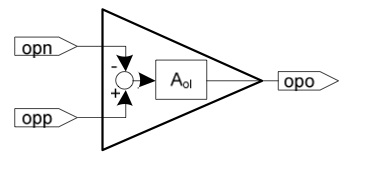
\includegraphics[width=0.4\linewidth]{images/op_ol.jpg}

\begin{align*}
A_{ol}(s) &= \frac{A_{ol,0}}{\left(1+\frac{s}{\omega_{\text{Pol}1}}\right)\left(1+\frac{s}{\omega_{\text{Pol}2}}\right)} = \frac{A_{ol,0}}{1 + \frac{A_{ol,0}}{2 \pi \text{GBP}}s}
\end{align*}

Betrachtung Op-Amp als Closed-Loop System: \\
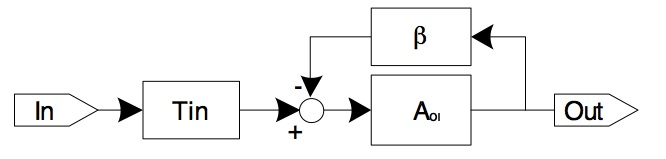
\includegraphics[width=0.8\linewidth]{images/op_feedback.jpg} \\
mit $\beta(s) = \frac{V_{\text{opn}}}{V_{out}}$, $T_{\In} = \frac{V_{\text{opn}}}{V_{\In}}$
ergibt sich

\begin{equation*}
	V_{\Out} = A_{cl}(s) V_{\In} = \frac{T_{\In} A_{ol}(s)}{1+A_{ol}(s) \beta(s)} V_{\In}
\end{equation*}
 
\end{multicols}


\begin{tabularx}{\linewidth}{llX}
	\textbf{Schaltung} & \textbf{Blockschaltbild} & \textbf{Berechnung} \\ \hline
	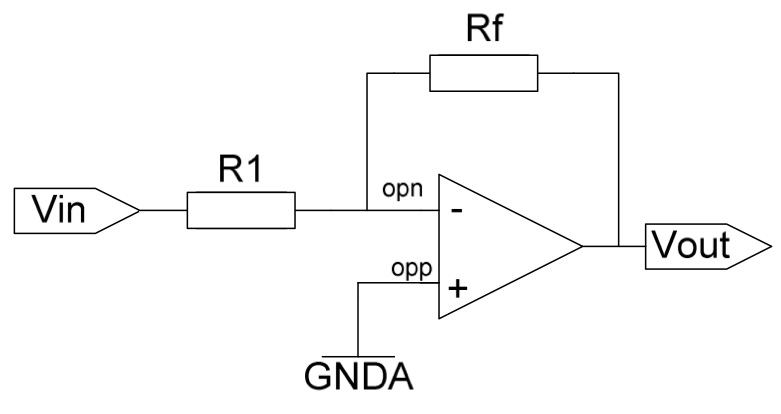
\includegraphics[width=4cm]{images/op_inv_sch.jpg} & 
	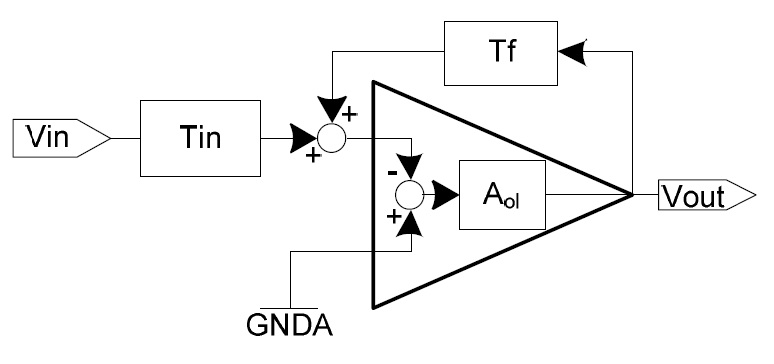
\includegraphics[width=4cm]{images/op_inv_block.jpg} & 
	$\beta = T_f = \frac{R_1}{R_1 + R_f}$ \newline
	$\frac{V_{\Out}}{V_{\In}} = -\frac{T_{\In}}{\beta} \frac{1}{1+\frac{1}{\beta A_{ol}}} \approx -\frac{R_f}{R_1} = \frac{1-\beta}{\beta}$ \\
	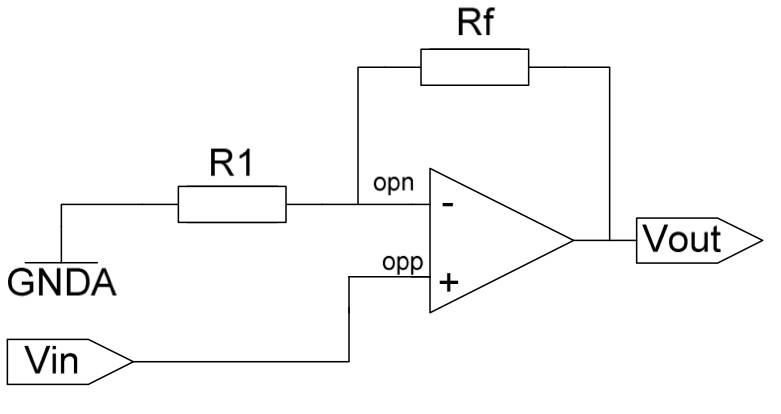
\includegraphics[width=4cm]{images/op_ninv_sch.jpg} & 
	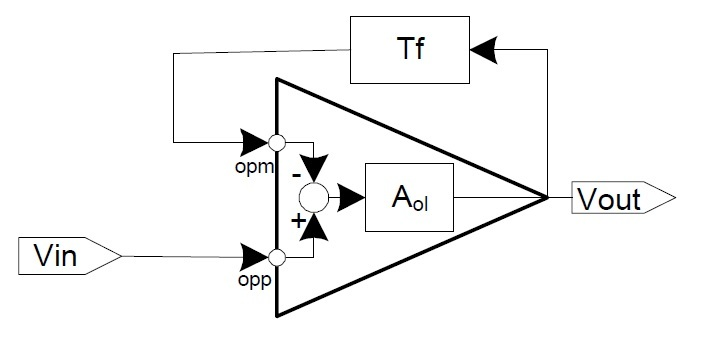
\includegraphics[width=4cm]{images/op_ninv_block.jpg} & 
	$\beta = T_f = \frac{R_1}{R_1 + R_f}$ \newline
	$\frac{V_{\Out}}{V_{\In}} = \frac{T_{\In}}{\beta} \frac{1}{1+\frac{1}{\beta A_{ol}}} \approx \frac{R_1 + R_f}{R_1} = \frac{1}{\beta} $\\ \hline
\end{tabularx}

